\documentclass[12pt,letterpaper]{article}
\usepackage{graphicx,textcomp}
\usepackage{natbib}
\usepackage{setspace}
\usepackage{fullpage}
\usepackage{color}
\usepackage[reqno]{amsmath}
\usepackage{amsthm}
\usepackage{fancyvrb}
\usepackage{amssymb,enumerate}
\usepackage[all]{xy}
\usepackage{endnotes}
\usepackage{lscape}
\newtheorem{com}{Comment}
\usepackage{float}
\usepackage{hyperref}
\newtheorem{lem} {Lemma}
\newtheorem{prop}{Proposition}
\newtheorem{thm}{Theorem}
\newtheorem{defn}{Definition}
\newtheorem{cor}{Corollary}
\newtheorem{obs}{Observation}
\usepackage[compact]{titlesec}
\usepackage{dcolumn}
\usepackage{tikz}
\usetikzlibrary{arrows}
\usepackage{multirow}
\usepackage{xcolor}
\newcolumntype{.}{D{.}{.}{-1}}
\newcolumntype{d}[1]{D{.}{.}{#1}}
\definecolor{light-gray}{gray}{0.65}
\usepackage{url}
\usepackage{listings}
\usepackage{color}

\definecolor{codegreen}{rgb}{0,0.6,0}
\definecolor{codegray}{rgb}{0.5,0.5,0.5}
\definecolor{codepurple}{rgb}{0.58,0,0.82}
\definecolor{backcolour}{rgb}{0.95,0.95,0.92}

\lstdefinestyle{mystyle}{
	backgroundcolor=\color{backcolour},   
	commentstyle=\color{codegreen},
	keywordstyle=\color{magenta},
	numberstyle=\tiny\color{codegray},
	stringstyle=\color{codepurple},
	basicstyle=\footnotesize,
	breakatwhitespace=false,         
	breaklines=true,                 
	captionpos=b,                    
	keepspaces=true,                 
	numbers=left,                    
	numbersep=5pt,                  
	showspaces=false,                
	showstringspaces=false,
	showtabs=false,                  
	tabsize=2
}
\lstset{style=mystyle}
\newcommand{\Sref}[1]{Section~\ref{#1}}
\newtheorem{hyp}{Hypothesis}

\title{Problem Set 3}
\date{Due: November 19, 2022}
\author{Applied Stats/Quant Methods 1}


\begin{document}
	\maketitle
	\section*{Instructions}
	\begin{itemize}
		\item Please show your work! You may lose points by simply writing in the answer. If the problem requires you to execute commands in \texttt{R}, please include the code you used to get your answers. Please also include the \texttt{.R} file that contains your code. If you are not sure if work needs to be shown for a particular problem, please ask.
	\item Your homework should be submitted electronically on GitHub.
	\item This problem set is due before 23:59 on Sunday November 19, 2023. No late assignments will be accepted.

	\end{itemize}

		\vspace{.25cm}
	
\noindent In this problem set, you will run several regressions and create an add variable plot (see the lecture slides) in \texttt{R} using the \texttt{incumbents\_subset.csv} dataset. Include all of your code.

	\vspace{.5cm}
\section*{Question 1}
\vspace{.25cm}
\noindent We are interested in knowing how the difference in campaign spending between incumbent and challenger affects the incumbent's vote share. 
	\begin{enumerate}
		\item Run a regression where the outcome variable is \texttt{voteshare} and the explanatory variable is \texttt{difflog}.	
		\subsection*{Answer.} 
		To run a regression where the outcome variable is voteshare and the explanatory variable is difflog the lm function in R can be used.
		\begin{lstlisting}[language=R]
			model1 <- lm(voteshare ~ difflog, data = inc.sub)
		\end{lstlisting}
		Where voteshare is the outcome (Y axis) variable and difflog is the explanatory (X axis) variable. Use the summary function to see the outcome of the linear regression model.
		The summary of the linear regression model1 is displayed on the below table:
		\vspace{5cm}
		\begin{table}[!htbp] \centering 
			\caption{} 
			\label{} 
			\begin{tabular}{@{\extracolsep{5pt}}lc} 
				\\[-1.8ex]\hline 
				\hline \\[-1.8ex] 
				& \multicolumn{1}{c}{\textit{Dependent variable:}} \\ 
				\cline{2-2} 
				\\[-1.8ex] & voteshare \\ 
				\hline \\[-1.8ex] 
				difflog & 0.042$^{***}$ \\ 
				& (0.001) \\ 
				& \\ 
				Constant & 0.579$^{***}$ \\ 
				& (0.002) \\ 
				& \\ 
				\hline \\[-1.8ex] 
				Observations & 3,193 \\ 
				R$^{2}$ & 0.367 \\ 
				Adjusted R$^{2}$ & 0.367 \\ 
				Residual Std. Error & 0.079 (df = 3191) \\ 
				F Statistic & 1,852.791$^{***}$ (df = 1; 3191) \\ 
				\hline 
				\hline \\[-1.8ex] 
				\textit{Note:}  & \multicolumn{1}{r}{$^{*}$p$<$0.1; $^{**}$p$<$0.05; $^{***}$p$<$0.01} \\ 
			\end{tabular} 
		\end{table} 
		\item Make a scatterplot of the two variables and add the regression line.
		\subsection*{Answer}
		To make a scatterplot of the linear model the following code can be used.
		\begin{lstlisting}[language=R]
{plot(voteshare ~ difflog, data = inc.sub, col = 'black')+
	abline(model1, col = 'red', lwd = 3)+
	grid()+
	title(main = 'Scatter Plot Voteshare Vs. Difflog', y = "voteshare",
	x = "difflog")
	}
		\end{lstlisting}
		Which produces the following scatterplot:
\begin{figure}[h]
	\centering
	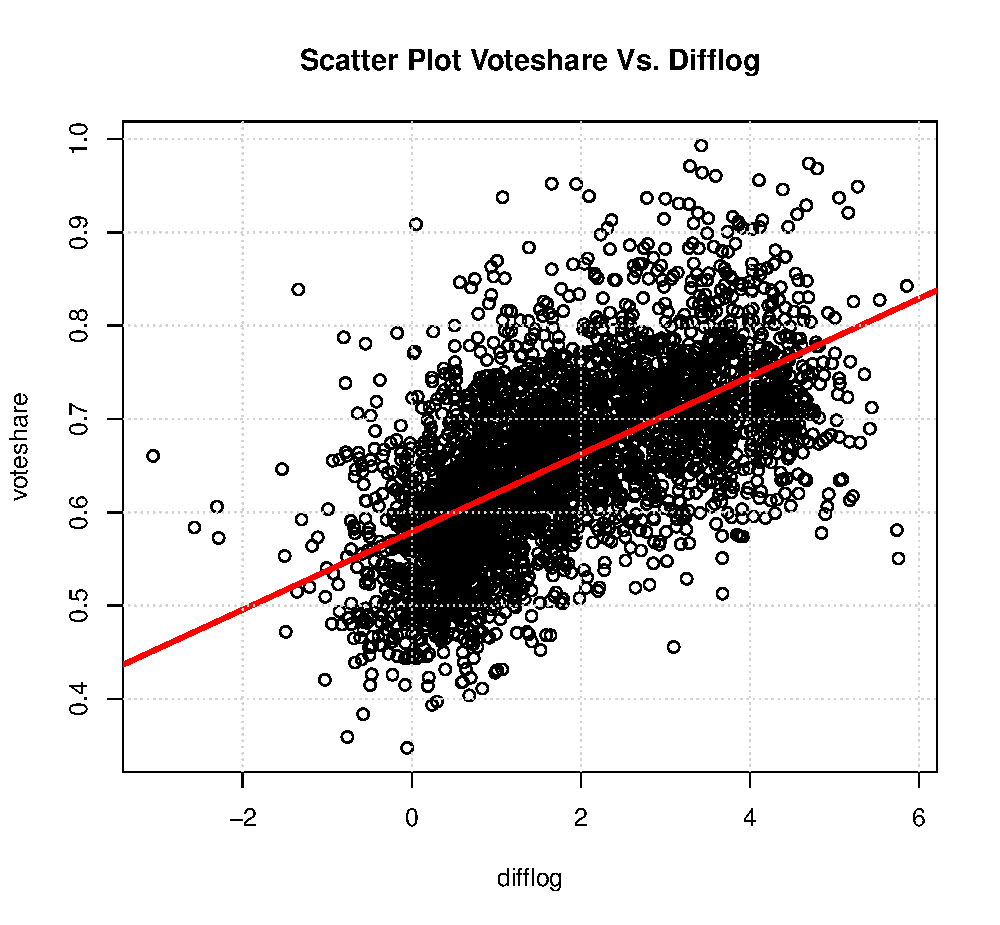
\includegraphics[width=0.75\textwidth]{SP_voteshare_v_difflog}
	\caption{Model 1}
	\label{fig:spvotesharevdifflog}
\end{figure}
\vspace{7cm}
		\item Save the residuals of the model in a separate object.	
		\subsection*{Answer.}
		To save the residuals of the model, "model1", in a separate object the following code can be used.
		\begin{lstlisting}[language=R]
			model1_residuals <- resid(model1)
		\end{lstlisting}
		The model residuals are now saved in a separate object called:
		\begin{Verbatim}
		"model1_residuals"
		\end{Verbatim}
		\item Write the prediction equation.
		\subsection*{Answer.}
		The prediction equation represents the relationship between an outcome variable and one or more explanatory variables. It can be written as such:
		
		\vspace{0.1cm}
		
		$\mu_y = \beta_0 + \beta_1 x_1 + \beta_2 x_2$...
		
		\vspace{0.1cm}
		
		Where:
		
		\vspace{0.1cm}
		
		$\mu_y$ = is the predicted mean of the outcome variable.
		
		\vspace{0.1cm}
		
		$\beta_0$ = Is the Y intercept (the value of the predicted mean of the outcome variable when the predictor variable is equal to 0).
		
		\vspace{0.1cm}
		
		$\beta_1$ = Is the slope of the regression line (the coefficient).
		
		\vspace{0.1cm}
		
		$x_1$ = Is the value of the predictor variable.
		
		\vspace{1cm}
		
		In the case of the linear regression model1, the prediction equation can be written:
		
		\vspace{0.1cm}
		
		\textbf{$\mu_y$ = (0.57903) + (0.04167 )*($x_1$)}
	\end{enumerate}
	
\newpage

\section*{Question 2}
\noindent We are interested in knowing how the difference between incumbent and challenger's spending and the vote share of the presidential candidate of the incumbent's party are related.	\vspace{.25cm}
	\begin{enumerate}
		\item Run a regression where the outcome variable is \texttt{presvote} and the explanatory variable is \texttt{difflog}.
		\subsection*{Answer.} 
		To run a regression where the outcome variable is presvote and the explanatory variable is difflog the lm function in R can be used.
		\begin{lstlisting}[language=R]
			model1 <- lm(presvote ~ difflog, data = inc.sub)
		\end{lstlisting}
		Where presvote is the outcome (Y axis) variable and difflog is the explanatory (X axis) variable. Use the summary function to see the outcome of the linear regression model.
		The summary of the linear regression model1 is displayed on the below table:
		\begin{table}[!htbp] \centering 
			\caption{} 
			\label{} 
			\begin{tabular}{@{\extracolsep{5pt}}lc} 
				\\[-1.8ex]\hline 
				\hline \\[-1.8ex] 
				& \multicolumn{1}{c}{\textit{Dependent variable:}} \\ 
				\cline{2-2} 
				\\[-1.8ex] & presvote \\ 
				\hline \\[-1.8ex] 
				difflog & 0.024$^{***}$ \\ 
				& (0.001) \\ 
				& \\ 
				Constant & 0.508$^{***}$ \\ 
				& (0.003) \\ 
				& \\ 
				\hline \\[-1.8ex] 
				Observations & 3,193 \\ 
				R$^{2}$ & 0.088 \\ 
				Adjusted R$^{2}$ & 0.088 \\ 
				Residual Std. Error & 0.110 (df = 3191) \\ 
				F Statistic & 307.715$^{***}$ (df = 1; 3191) \\ 
				\hline 
				\hline \\[-1.8ex] 
				\textit{Note:}  & \multicolumn{1}{r}{$^{*}$p$<$0.1; $^{**}$p$<$0.05; $^{***}$p$<$0.01} \\ 
			\end{tabular} 
		\end{table} 
			\vspace{5cm}
		\item Make a scatterplot of the two variables and add the regression line.
		\subsection*{Answer}
		To make a scatterplot of the linear model the following code can be used.
		\begin{lstlisting}[language=R]
{plot(presvote ~ difflog, data = inc.sub, col = 'black')+
	abline(model2, col = 'red', lwd = 3)+
	grid()+
	title(main = 'Scatter Plot Presvote Vs. Difflog', y = "presvote",
	 x = "difflog")
}
		\end{lstlisting}
		Which produces the following scatterplot:
		
		\vspace{0.5cm}
		
\begin{figure}[h]
	\centering
	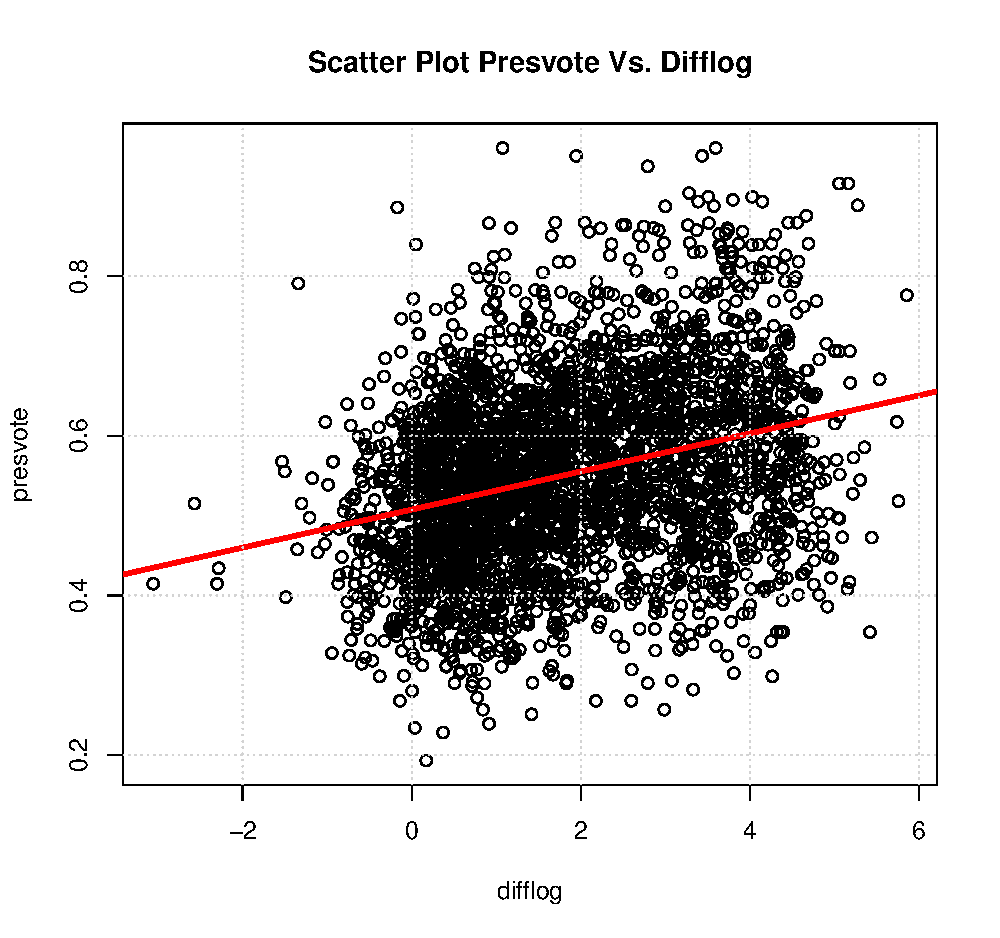
\includegraphics[width=0.75\textwidth]{SP_presvote_v_difflog}
	\caption{Model 2}
	\label{fig:sppresvotevdifflog}
\end{figure}
\newpage
		\item Save the residuals of the model in a separate object.
		\subsection*{Answer.}
		To save the residuals of the model, "model2", in a separate object the following code can be used.
		\begin{lstlisting}[language=R]
			model2_residuals <- resid(model2)
		\end{lstlisting}
		The model residuals are now saved in a separate object called:
		\begin{Verbatim}
			"model2_residuals"
		\end{Verbatim}
		
		\vspace{4cm}
		\item Write the prediction equation.
		
		\vspace{0.1cm}
		
		The prediction equation for model2 can be written as:\footnote{Refer to Question 1, part 4 for an explanation of the  prediction equation.}
		
		\vspace{0.1cm}
		
		\textbf{$\mu_y$ = (0.50758) + (0.02384)*($x_1$)}
	\end{enumerate}
	
	\newpage	
\section*{Question 3}

\noindent We are interested in knowing how the vote share of the presidential candidate of the incumbent's party is associated with the incumbent's electoral success.
	\vspace{.25cm}
	\begin{enumerate}
		\item Run a regression where the outcome variable is \texttt{voteshare} and the explanatory variable is \texttt{presvote}.
		\subsection*{Answer.} 
		To run a regression where the outcome variable is voteshare and the explanatory variable is presvote the lm function in R can be used.
		\begin{lstlisting}[language=R]
			model3 <- lm(voteshare ~ presvote, data = inc.sub)
		\end{lstlisting}
		Where voteshare is the outcome (Y axis) variable and presvote is the explanatory (X axis) variable. The summary of the linear regression model3 is displayed on the below table:
		\begin{table}[!htbp] \centering 
			\caption{} 
			\label{} 
			\begin{tabular}{@{\extracolsep{5pt}}lc} 
				\\[-1.8ex]\hline 
				\hline \\[-1.8ex] 
				& \multicolumn{1}{c}{\textit{Dependent variable:}} \\ 
				\cline{2-2} 
				\\[-1.8ex] & voteshare \\ 
				\hline \\[-1.8ex] 
				presvote & 0.388$^{***}$ \\ 
				& (0.013) \\ 
				& \\ 
				Constant & 0.441$^{***}$ \\ 
				& (0.008) \\ 
				& \\ 
				\hline \\[-1.8ex] 
				Observations & 3,193 \\ 
				R$^{2}$ & 0.206 \\ 
				Adjusted R$^{2}$ & 0.206 \\ 
				Residual Std. Error & 0.088 (df = 3191) \\ 
				F Statistic & 826.950$^{***}$ (df = 1; 3191) \\ 
				\hline 
				\hline \\[-1.8ex] 
				\textit{Note:}  & \multicolumn{1}{r}{$^{*}$p$<$0.1; $^{**}$p$<$0.05; $^{***}$p$<$0.01} \\ 
			\end{tabular} 
		\end{table} 
			\vspace{5cm}
		\item Make a scatterplot of the two variables and add the regression line. 
			\subsection*{Answer}
		To make a scatterplot of the linear model the following code can be used.
		\begin{lstlisting}[language=R]
{plot(voteshare ~ presvote, data = inc.sub, col = 'black')+
	abline(model3, col = 'red', lwd = 3)+
	grid()+
	title(main = 'Scatter Plot Voteshare Vs. Presvote', y = "voteshare",
	x = "presvote")
}
		\end{lstlisting}
		Which produces the following scatterplot:
\begin{figure}[h]
	\centering
	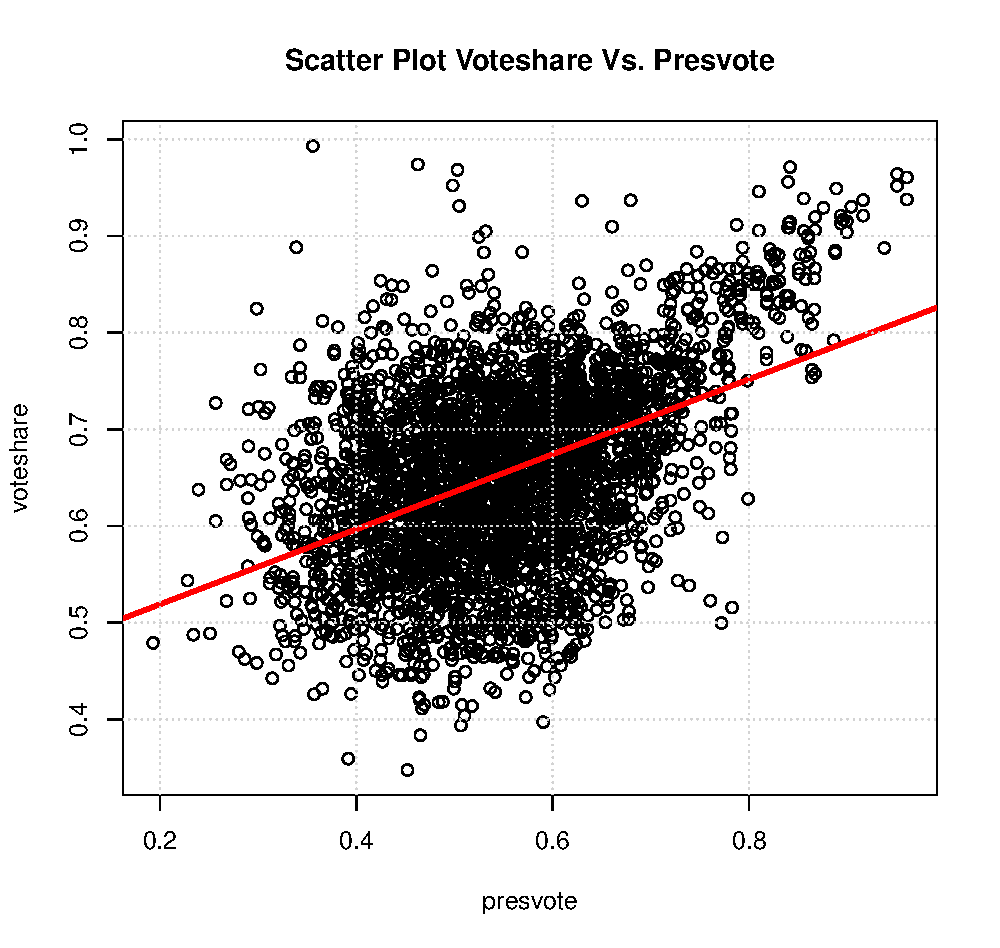
\includegraphics[width=0.75\textwidth]{SP_voteshare_v_presvote}
	\caption{Model 3}
	\label{fig:spvotesharevpresvote}
\end{figure}
			\vspace{5cm}
		\item Write the prediction equation.
		\subsection*{Answer.}
		\vspace{0.1cm}
		
		The prediction equation for model3 can be written as:\footnote{Refer to Question 1, part 4 for an explanation of the  prediction equation.}
		
		\vspace{0.1cm}
		
			\textbf{$\mu_y$ = (0.4413) + (0.3880)*($x_1$)}
	\end{enumerate}
	

\newpage	
\section*{Question 4}
\noindent The residuals from part (a) tell us how much of the variation in \texttt{voteshare} is $not$ explained by the difference in spending between incumbent and challenger. The residuals in part (b) tell us how much of the variation in \texttt{presvote} is $not$ explained by the difference in spending between incumbent and challenger in the district.
	\begin{enumerate}
		\item Run a regression where the outcome variable is the residuals from Question 1 and the explanatory variable is the residuals from Question 2.
		\subsection*{Answer.}
		To run a regression where the outcome variable is the residuals from Question 1 and the explanatory variable is the residuals from Question 2 the residuals must first be saved in a dataframe together, which can be done with the following code.
		\begin{lstlisting}[language=R]
{df1 <- as.data.frame(model1_residuals)
	df2 <- as.data.frame(model2_residuals)
	list_df3 <- c(df1, df2)
	df3 <- as.data.frame(list_df3)
}
		\end{lstlisting}
		Now the residuals from both Questions are saved in a common dataframe called 'df3'. A linear regression can be run on the residuals from Questions 1 and 2 with the lm function.
			\begin{lstlisting}[language=R]
model4 <- lm(model1_residuals ~ model2_residuals, data = df3)
		\end{lstlisting}
		Where model1 residuals  is the outcome (Y axis) variable and model2 residuals is the explanatory (X axis) variable. The summary of the linear regression model3 is displayed on the below table:
		\begin{table}[!htbp] \centering 
			\caption{} 
			\label{} 
			\begin{tabular}{@{\extracolsep{5pt}}lc} 
				\\[-1.8ex]\hline 
				\hline \\[-1.8ex] 
				& \multicolumn{1}{c}{\textit{Dependent variable:}} \\ 
				\cline{2-2} 
				\\[-1.8ex] & model1\_residuals \\ 
				\hline \\[-1.8ex] 
				model2\_residuals & 0.257$^{***}$ \\ 
				& (0.012) \\ 
				& \\ 
				Constant & $-$0.000 \\ 
				& (0.001) \\ 
				& \\ 
				\hline \\[-1.8ex] 
				Observations & 3,193 \\ 
				R$^{2}$ & 0.130 \\ 
				Adjusted R$^{2}$ & 0.130 \\ 
				Residual Std. Error & 0.073 (df = 3191) \\ 
				F Statistic & 476.975$^{***}$ (df = 1; 3191) \\ 
				\hline 
				\hline \\[-1.8ex] 
				\textit{Note:}  & \multicolumn{1}{r}{$^{*}$p$<$0.1; $^{**}$p$<$0.05; $^{***}$p$<$0.01} \\ 
			\end{tabular} 
		\end{table} 
		\vspace{9cm}
		\item Make a scatterplot of the two residuals and add the regression line.
		\subsection*{Answer.}
		
		 
		To make a scatterplot of the linear regression with a regression line the following code can be used:
		\begin{lstlisting}[language=R]
		{plot(model1_residuals ~ model2_residuals, data = df3, col = 'black')+
			abline(model4, col = 'red', lwd = 3)+
			grid()+
			title(main = 'Scatter Plot model1_residuals Vs. model2_residuals', y = "model1_residuals", x = "model2_residuals")
		}
		\end{lstlisting}
		\newpage
		Which produces this scatterplot:
\begin{figure}[h]
	\centering
	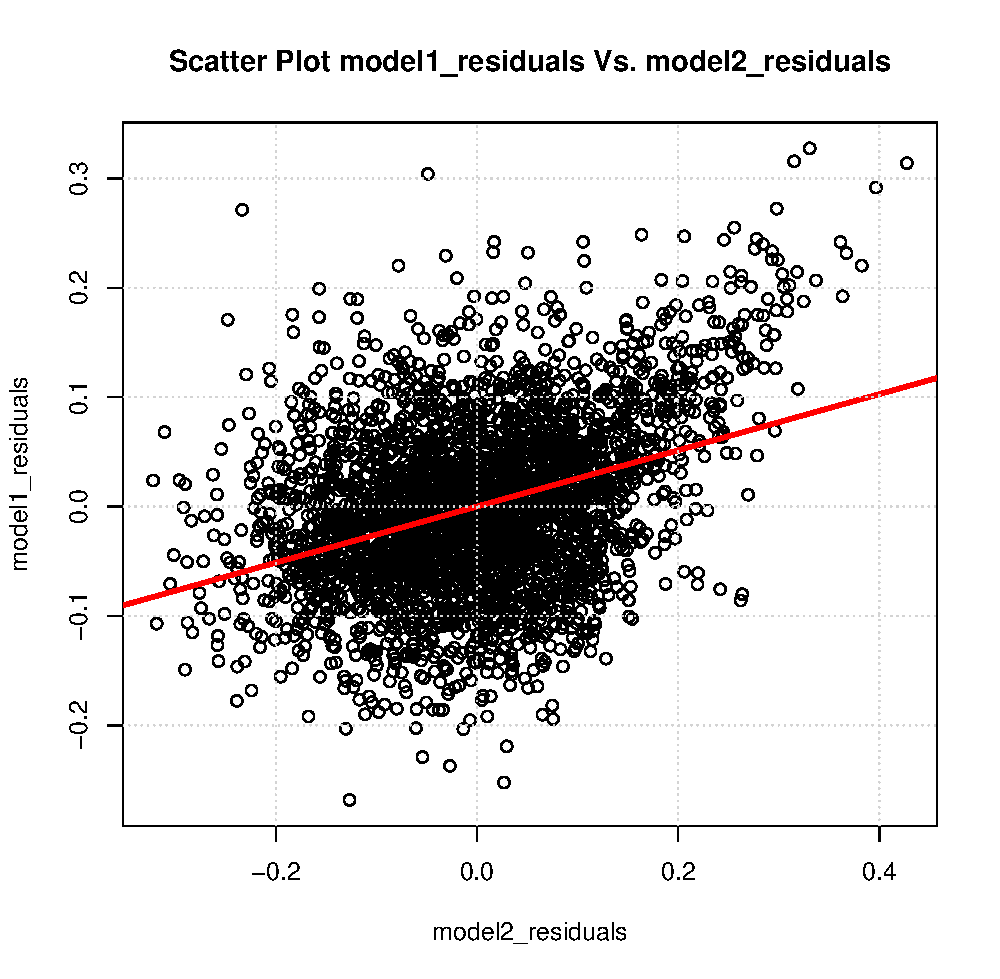
\includegraphics[width=0.75\textwidth]{SP_m1r_v_m2r}
	\caption{Model 4}
	\label{fig:spm1rvm2r}
\end{figure}
		\item Write the prediction equation.
		\subsection*{Answer.}
		The prediction equation for model4 can be written as:\footnote{Refer to Question 1, part 4 for an explanation of the  prediction equation.}
		
		\vspace{0.1cm}
		
		\textbf{$\mu_y$ = (-5.934e-18) + (2.569e-01)*($x_1$)}
	\end{enumerate}
	
	\newpage	

\section*{Question 5}
\noindent What if the incumbent's vote share is affected by both the president's popularity and the difference in spending between incumbent and challenger? 
	\begin{enumerate}
		\item Run a regression where the outcome variable is the incumbent's \texttt{voteshare} and the explanatory variables are \texttt{difflog} and \texttt{presvote}.
		\subsection*{Answer.}
		To run a regression where the outcome variable is the incumbent's voteshare and the explanatory variables are difflog and presvote the lm function can be used in R.
		
		\vspace{0.5cm}
		\begin{lstlisting}[language=R]
	model5 <- lm(voteshare ~ difflog + presvote, data = inc.sub)
		\end{lstlisting}
		A summary of the linear regression model5 can be viewed on the table below.
		\begin{table}[!htbp] \centering 
			\caption{} 
			\label{} 
			\begin{tabular}{@{\extracolsep{5pt}}lc} 
				\\[-1.8ex]\hline 
				\hline \\[-1.8ex] 
				& \multicolumn{1}{c}{\textit{Dependent variable:}} \\ 
				\cline{2-2} 
				\\[-1.8ex] & voteshare \\ 
				\hline \\[-1.8ex] 
				difflog & 0.036$^{***}$ \\ 
				& (0.001) \\ 
				& \\ 
				presvote & 0.257$^{***}$ \\ 
				& (0.012) \\ 
				& \\ 
				Constant & 0.449$^{***}$ \\ 
				& (0.006) \\ 
				& \\ 
				\hline \\[-1.8ex] 
				Observations & 3,193 \\ 
				R$^{2}$ & 0.450 \\ 
				Adjusted R$^{2}$ & 0.449 \\ 
				Residual Std. Error & 0.073 (df = 3190) \\ 
				F Statistic & 1,302.947$^{***}$ (df = 2; 3190) \\ 
				\hline 
				\hline \\[-1.8ex] 
				\textit{Note:}  & \multicolumn{1}{r}{$^{*}$p$<$0.1; $^{**}$p$<$0.05; $^{***}$p$<$0.01} \\ 
			\end{tabular} 
		\end{table} 	\vspace{5cm}
		\item Write the prediction equation.
		\subsection*{Answer.}
		The prediction equation for model5 can be written as: \footnote{Refer to Question 1, part 4 for an explanation of the prediction equation.}
		
		\vspace{0.1cm}
		
		\textbf{$\mu_y$ = (0.44864) + (0.03554)*($x_1$) + (0.25688)*($x_2$)}
		
		\vspace{2cm}
		
		\item What is it in this output that is identical to the output in Question 4? Why do you think this is the case?
		\subsection*{Answer.}
		The standard residual error in both model4 and model5 are identical, it is equal to 0.073 in both cases.
		
		\vspace{0.1cm}
		
		A standardized residual in a linear regression model is the difference between a predicted value and an observed value in the model. The standard residual error is the value assigned to the error of the model as a whole, it is used to quantify the variability of the observed data points around a fitted regression line.
		
		\vspace{0.1cm}
		
		When model4 and model5 are printed in R, it seems as though the intercept value assigned to model2-residuals (in model4) and presvote (in model5) is very similar, this can also be viewed in tables 4 and 5, where the value is 0.257 for both model2-residuals (in model4) and presvote (in model5). The correlation of these values can be calculated in R with the cor function.
		\begin{lstlisting}[language=R]
			cor(model2_residuals, inc.sub$presvote)
		\end{lstlisting}
		Which returns a value of 0.9550126, suggesting they are very highly correlated.
		
		\vspace{0.1cm}
		
		Model1 is the regression of voteshare vs difflog, where voteshare is the outcome variable. The residuals of this model tell how much of the variation in voteshare is not explained by difflog.
		
		\vspace{0.1cm}
		
		Model2 is the regression of presvote vs difflog, where presvote is the outcome variable. The residuals of this model tell how much of the variation in presvote is not explained by difflog (the difference in spending between the incumbent and the challenger). 
		
		\vspace{0.1cm}
		
		Model4 is a regression of the residuals of both these models, model1-residuals vs model2-residuals, where model1-residuals is the outcome variable. The residuals from this model tell how much of of the variation in model1-residuals is not explained by model2-residuals.
		
		\vspace{0.1cm}
		
		Model5 is a regression of voteshare vs difflog + presvote. Where voteshare is the outcome variable. The residuals from this model tell how much of the variation in voteshare is not explained by both difflog + presvote.
		
		In the regression model1-residuals vs model2-residuals, 0.257 is the slope of the their line of best fit. In the regression voteshare vs presvote + difflog 0.257 is the slope of the line of best fit between presvote and voteshare. Both regressions contain the same variables interacting in similar ways, the variable difflog cancels out, this is why they have a very highly correlated standard residual error. 
	\end{enumerate}

\section*{Bibliography}
\begin{itemize}
	\item Dr. Jeffery Ziegler's lecture slides.
	\item Hannah Frank's tutorial material.
	\item Zach (2021) ‘How to Interpret Residual Standard Error’, Statology, 11 May. Available at: https://www.statology.org/how-to-interpret-residual-standard-error/ (Accessed: 19 November 2023).
	\item Residual Standard Error (RSE) (2018). Available at: https://www.youtube.com/watch?v=rLwn7OKcoqk (Accessed: 19 November 2023).
	\item Zach (2020) ‘What Are Standardized Residuals?’, Statology, 22 December. Available at: https://www.statology.org/standardized-residuals/ (Accessed: 19 November 2023).
	
\end{itemize}




\end{document}
